\documentclass[a4paper,11pt]{article}
\usepackage[T1]{fontenc}
\usepackage[utf8]{inputenc}
\usepackage[margin=2.5cm]{geometry}
\usepackage{graphicx}
\usepackage{booktabs}
\usepackage{amsmath}
\usepackage{amssymb}
\usepackage{lineno}
\usepackage[hidelinks]{hyperref}

% All numerical results quoted in the text are generated from the selected campaign artifacts
% by scripts/build_revision_figures.py (see generated/figure_provenance.csv).
% Generated by scripts/build_revision_figures.py; do not edit.
\newcommand{\AccPoints}{3692}
\newcommand{\AlignedMomentX}{$4.5\times10^{-7}$}
\newcommand{\AlignedMomentY}{$1.6\times10^{-7}$}
\newcommand{\AmpThinMinus}{+0.66}
\newcommand{\AmpThinNom}{9.07}
\newcommand{\AmpThinPlus}{+1.22}
\newcommand{\AmpThreeDMinus}{+0.60}
\newcommand{\AmpThreeDNom}{9.57}
\newcommand{\AmpThreeDPlus}{-0.12}
\newcommand{\AperDiagNoVert}{88.0}
\newcommand{\AperDiagOpenNoVert}{94.8}
\newcommand{\AperDiagRef}{93.0}
\newcommand{\AperDiagXopen}{86.3}
\newcommand{\AperDiagYten}{92.4}
\newcommand{\AperElevenCap}{76.0}
\newcommand{\AperFifteenCap}{86.3}
\newcommand{\AperTenCap}{47.9}
\newcommand{\AperTwelveCap}{83.8}
\newcommand{\ArcNormY}{1.81}
\newcommand{\BicubicErr}{$9\times10^{-11}$}
\newcommand{\BigCap}{92.4}
\newcommand{\BigHi}{93.5}
\newcommand{\BigLo}{91.2}
\newcommand{\BigLossCreation}{0}
\newcommand{\BigLossElsewhere}{135}
\newcommand{\BigLossMagnet}{0}
\newcommand{\BigLossSeptumReturn}{17}
\newcommand{\BigN}{2000}
\newcommand{\BilinearErr}{$1\times10^{-6}$}
\newcommand{\BudBetaMis}{5}
\newcommand{\BudDipB}{0.05}
\newcommand{\BudEmit}{10}
\newcommand{\BudEnergy}{0.1}
\newcommand{\BudEspread}{1}
\newcommand{\BudJitX}{0.5}
\newcommand{\BudJitXp}{0.2}
\newcommand{\BudNkmDx}{0.2}
\newcommand{\BudNkmScale}{0.5}
\newcommand{\BudNkmTiming}{0.1}
\newcommand{\BudQuadDx}{100}
\newcommand{\BudQuadK}{0.1}
\newcommand{\BudQuadRoll}{0.5}
\newcommand{\BudRingCo}{0.2}
\newcommand{\BudSeptum}{0.1}
\newcommand{\CapThickOneD}{87.4}
\newcommand{\CapThinLegacy}{91.1}
\newcommand{\CapThinPhys}{89.7}
\newcommand{\CapThreeDNoVert}{87.8}
\newcommand{\CapThreeDRematch}{81.8}
\newcommand{\CapThreeDSame}{84.8}
\newcommand{\CapThreeDVertDiag}{82.5}
\newcommand{\CentreNormY}{2.64}
\newcommand{\ChamberDAFirstMax}{-7.0}
\newcommand{\ChamberDAFirstMin}{-10.0}
\newcommand{\ChamberDiff}{-0.3}
\newcommand{\ChamberDiffHi}{+0.3}
\newcommand{\ChamberDiffLo}{-0.9}
\newcommand{\ChamberDipole}{97.3}
\newcommand{\ChamberGridFifteen}{99.7}
\newcommand{\ChamberGridTen}{81.7}
\newcommand{\ChamberGridTwelve}{97.0}
\newcommand{\ChamberIdealDANeg}{-11.0}
\newcommand{\ChamberIdealDAPos}{12.5}
\newcommand{\ChamberNom}{97.0}
\newcommand{\ChamberNomHi}{97.9}
\newcommand{\ChamberNomLo}{95.7}
\newcommand{\ChamberRingMax}{87.4}
\newcommand{\ChamberRingMean}{61.7}
\newcommand{\ChamberRingMedian}{63.7}
\newcommand{\ChamberRingMin}{2.7}
\newcommand{\ChamberRingPten}{52.3}
\newcommand{\ClosedIvuNormY}{1.31}
\newcommand{\CtrlDipoleAmp}{2495}
\newcommand{\CubicCoeff}{$2.4\times10^{4}$}
\newcommand{\DAxMaxMm}{13}
\newcommand{\DAxMinMm}{-12}
\newcommand{\DeltaSensUrad}{0.12}
\newcommand{\DipoleResidualRel}{$4\times10^{-5}$}
\newcommand{\EightUsResidual}{0.50}
\newcommand{\EmitFiftyCap}{97.4}
\newcommand{\EmitHundredCap}{93.1}
\newcommand{\EmitOneFiftyCap}{87.2}
\newcommand{\EmitTwentyFiveCap}{98.9}
\newcommand{\EmitTwoHundredCap}{81.1}
\newcommand{\EmitYRatio}{0.1}
\newcommand{\FinalAlphaC}{7.77\times10^{-5}}
\newcommand{\FinalAngleHi}{0.24}
\newcommand{\FinalAngleLo}{-0.52}
\newcommand{\FinalAngleWidth}{0.76}
\newcommand{\FinalBackendLinear}{100.0}
\newcommand{\FinalBackendNative}{97.0}
\newcommand{\FinalBackendTangentMax}{1.36\times10^{-14}}
\newcommand{\FinalControlDiff}{-7.7}
\newcommand{\FinalControlDiffHi}{-5.4}
\newcommand{\FinalControlDiffLo}{-10.3}
\newcommand{\FinalDampingXMs}{10.54}
\newcommand{\FinalDampingYMs}{19.43}
\newcommand{\FinalDampingZMs}{16.79}
\newcommand{\FinalDegradedLong}{1.4}
\newcommand{\FinalDegradedLongHi}{2.3}
\newcommand{\FinalDegradedLongLo}{0.8}
\newcommand{\FinalDegradedShort}{3.0}
\newcommand{\FinalDipAboveEighty}{5.3}
\newcommand{\FinalDipHi}{27.0}
\newcommand{\FinalDipLo}{18.3}
\newcommand{\FinalDipMean}{22.5}
\newcommand{\FinalDipMedian}{7.8}
\newcommand{\FinalDipPten}{0.0}
\newcommand{\FinalInjectedBunchMm}{13.4}
\newcommand{\FinalInjectedEmitNm}{7.67}
\newcommand{\FinalJitterFullAboveEighty}{4.0}
\newcommand{\FinalJitterFullDiff}{-14.3}
\newcommand{\FinalJitterFullDiffHi}{-7.8}
\newcommand{\FinalJitterFullDiffLo}{-21.3}
\newcommand{\FinalJitterFullMean}{19.8}
\newcommand{\FinalJitterFullMedian}{3.5}
\newcommand{\FinalJitterFullPten}{0.0}
\newcommand{\FinalJitterHalfAboveEighty}{4.0}
\newcommand{\FinalJitterHalfDiff}{-4.7}
\newcommand{\FinalJitterHalfDiffHi}{+0.0}
\newcommand{\FinalJitterHalfDiffLo}{-9.6}
\newcommand{\FinalJitterHalfMean}{29.4}
\newcommand{\FinalJitterHalfMedian}{24.0}
\newcommand{\FinalJitterHalfPten}{0.0}
\newcommand{\FinalJitterQuarterAboveEighty}{6.0}
\newcommand{\FinalJitterQuarterDiff}{+2.2}
\newcommand{\FinalJitterQuarterDiffHi}{+6.1}
\newcommand{\FinalJitterQuarterDiffLo}{-1.5}
\newcommand{\FinalJitterQuarterMean}{36.3}
\newcommand{\FinalJitterQuarterMedian}{31.5}
\newcommand{\FinalJitterQuarterPten}{0.0}
\newcommand{\FinalJitterRows}{0 & 34.1 & 28.2 & 0.0 & 4 & +0.0 & [+0.0, +0.0] \\
0.25 & 36.3 & 31.5 & 0.0 & 6 & +2.2 & [-1.5, +6.1] \\
0.5 & 29.4 & 24.0 & 0.0 & 4 & -4.7 & [-9.6, +0.0] \\
0.75 & 22.9 & 7.0 & 0.0 & 4 & -11.2 & [-17.8, -5.2] \\
1 & 19.8 & 3.5 & 0.0 & 4 & -14.3 & [-21.3, -7.8] \\
position only & 30.8 & 21.5 & 0.0 & 6 & -3.3 & [-8.5, +1.5] \\
angle only & 20.8 & 3.8 & 0.0 & 6 & -13.2 & [-19.6, -7.2] \\}
\newcommand{\FinalJitterXonlyAboveEighty}{6.0}
\newcommand{\FinalJitterXonlyDiff}{-3.3}
\newcommand{\FinalJitterXonlyDiffHi}{+1.5}
\newcommand{\FinalJitterXonlyDiffLo}{-8.5}
\newcommand{\FinalJitterXonlyMean}{30.8}
\newcommand{\FinalJitterXonlyMedian}{21.5}
\newcommand{\FinalJitterXonlyPten}{0.0}
\newcommand{\FinalJitterXponlyAboveEighty}{6.0}
\newcommand{\FinalJitterXponlyDiff}{-13.2}
\newcommand{\FinalJitterXponlyDiffHi}{-7.2}
\newcommand{\FinalJitterXponlyDiffLo}{-19.6}
\newcommand{\FinalJitterXponlyMean}{20.8}
\newcommand{\FinalJitterXponlyMedian}{3.8}
\newcommand{\FinalJitterXponlyPten}{0.0}
\newcommand{\FinalJitterZeroAboveEighty}{4.0}
\newcommand{\FinalJitterZeroDiff}{+0.0}
\newcommand{\FinalJitterZeroDiffHi}{+0.0}
\newcommand{\FinalJitterZeroDiffLo}{+0.0}
\newcommand{\FinalJitterZeroMean}{34.1}
\newcommand{\FinalJitterZeroMedian}{28.2}
\newcommand{\FinalJitterZeroPten}{0.0}
\newcommand{\FinalLateLoss}{0.9}
\newcommand{\FinalLong}{96.1}
\newcommand{\FinalLongHi}{97.1}
\newcommand{\FinalLongLo}{94.7}
\newcommand{\FinalLowerLong}{79.4}
\newcommand{\FinalLowerLongHi}{81.8}
\newcommand{\FinalLowerLongLo}{76.8}
\newcommand{\FinalLowerShort}{79.5}
\newcommand{\FinalNkmAboveEighty}{2.7}
\newcommand{\FinalNkmHi}{18.8}
\newcommand{\FinalNkmLo}{11.2}
\newcommand{\FinalNkmMean}{14.8}
\newcommand{\FinalNkmMedian}{1.0}
\newcommand{\FinalNkmPten}{0.0}
\newcommand{\FinalPositionHi}{1.32}
\newcommand{\FinalPositionLo}{-0.67}
\newcommand{\FinalPositionWidth}{1.99}
\newcommand{\FinalRFfreqMHz}{499.593}
\newcommand{\FinalRFvoltageMV}{3.08}
\newcommand{\FinalRankRows}{booster\_xp\_rad & -0.51 & 1.16e-09 & 2.2e-08 \\
energy\_dp\_p & -0.15 & 0.109 & 1 \\
rms\_quad\_dy\_m & -0.14 & 0.116 & 1 \\
rms\_quad\_dx\_m & -0.13 & 0.143 & 1 \\
septum\_x\_m & -0.12 & 0.183 & 1 \\
nkm\_dx\_m & -0.10 & 0.281 & 1 \\
booster\_x\_m & -0.09 & 0.323 & 1 \\
nkm\_scale\_err & -0.05 & 0.613 & 1 \\
rf\_phase\_rad & -0.03 & 0.773 & 1 \\
rms\_quad\_roll\_rad & -0.03 & 0.776 & 1 \\
rms\_quad\_k\_err & -0.02 & 0.797 & 1 \\
dipole\_b\_err & -0.01 & 0.935 & 1 \\
septum\_strength\_rel & -0.01 & 0.953 & 1 \\
beta\_mismatch\_x & -0.00 & 0.995 & 1 \\
arrival\_time\_s & +0.02 & 0.829 & 1 \\
ring\_co\_x\_m & +0.03 & 0.714 & 1 \\
espread\_abs & +0.05 & 0.577 & 1 \\
emit\_rel & +0.05 & 0.562 & 1 \\
beta\_mismatch\_y & +0.07 & 0.472 & 1 \\}
\newcommand{\FinalRankSummary}{The smallest Holm-adjusted probabilities below 0.05 correspond to booster angle ($\rho=-0.51$, $p_\mathrm{Holm}=2.20\times10^{-8}$).}
\newcommand{\FinalSourceElements}{3481}
\newcommand{\FinalStoredBunchMm}{3.63}
\newcommand{\FinalSynchTune}{3.44\times10^{-3}}
\newcommand{\FinalTuneQuarterAboveEighty}{10.0}
\newcommand{\FinalTuneQuarterGain}{+5.5}
\newcommand{\FinalTuneQuarterGainHi}{+10.0}
\newcommand{\FinalTuneQuarterGainLo}{+1.1}
\newcommand{\FinalTuneQuarterMean}{41.8}
\newcommand{\FinalTuneQuarterMedian}{47.5}
\newcommand{\FinalTuneQuarterPten}{0.0}
\newcommand{\FinalTuneZeroAboveEighty}{12.0}
\newcommand{\FinalTuneZeroGain}{+11.6}
\newcommand{\FinalTuneZeroGainHi}{+15.5}
\newcommand{\FinalTuneZeroGainLo}{+7.8}
\newcommand{\FinalTuneZeroMean}{45.7}
\newcommand{\FinalTuneZeroMedian}{53.8}
\newcommand{\FinalTuneZeroPten}{0.0}
\newcommand{\FinalUpperLong}{84.7}
\newcommand{\FinalUpperLongHi}{86.8}
\newcommand{\FinalUpperLongLo}{82.3}
\newcommand{\FinalUpperShort}{85.0}
\newcommand{\GenAllowFraction}{91}
\newcommand{\GenAllowMrad}{0.076}
\newcommand{\GenConfigs}{30}
\newcommand{\GenEtaMax}{0.098}
\newcommand{\GenEtaMin}{0.005}
\newcommand{\GenEtaStar}{0.036}
\newcommand{\GenExpFamilyOne}{1.47}
\newcommand{\GenExpFamilyTwo}{1.45}
\newcommand{\GenExpX}{1.46}
\newcommand{\GenExpY}{0.81}
\newcommand{\GenNomEta}{0.034}
\newcommand{\GenNomThinDpx}{0.069}
\newcommand{\GenNomThinDpy}{0.129}
\newcommand{\GenNomW}{9.4}
\newcommand{\GenPrefX}{1.95}
\newcommand{\GenScatterMaxX}{11}
\newcommand{\GenScatterX}{3.4}
\newcommand{\GenScatterY}{7}
\newcommand{\GenSlicedMax}{$2\times10^{-5}$}
\newcommand{\GradResidualRel}{$7\times10^{-5}$}
\newcommand{\GridParticles}{200}
\newcommand{\GridPoints}{27}
\newcommand{\GridSkipped}{15}
\newcommand{\InjSigmaXmm}{0.50}
\newcommand{\InjSigmaXpMrad}{0.21}
\newcommand{\JitCFullFracEighty}{18}
\newcommand{\JitCFullHi}{55.7}
\newcommand{\JitCFullLo}{39.2}
\newcommand{\JitCFullMean}{47.3}
\newcommand{\JitCFullMedian}{48.5}
\newcommand{\JitCFullPten}{5.8}
\newcommand{\JitCHalfFracEighty}{36}
\newcommand{\JitCHalfHi}{70.4}
\newcommand{\JitCHalfLo}{56.7}
\newcommand{\JitCHalfMean}{63.6}
\newcommand{\JitCHalfMedian}{69.0}
\newcommand{\JitCHalfPten}{27.7}
\newcommand{\JitCQuarterFracEighty}{56}
\newcommand{\JitCQuarterHi}{76.4}
\newcommand{\JitCQuarterLo}{63.1}
\newcommand{\JitCQuarterMean}{70.0}
\newcommand{\JitCQuarterMedian}{81.2}
\newcommand{\JitCQuarterPten}{38.4}
\newcommand{\JitCRemovalGain}{22.4}
\newcommand{\JitCRemovalGainHi}{29.5}
\newcommand{\JitCRemovalGainLo}{15.7}
\newcommand{\JitCScaleForEighty}{none}
\newcommand{\JitCScaleForEightyHi}{none}
\newcommand{\JitCScaleForEightyLo}{none}
\newcommand{\JitCThreeQFracEighty}{24}
\newcommand{\JitCThreeQHi}{63.4}
\newcommand{\JitCThreeQLo}{48.1}
\newcommand{\JitCThreeQMean}{55.8}
\newcommand{\JitCThreeQMedian}{58.5}
\newcommand{\JitCThreeQPten}{19.5}
\newcommand{\JitCXOnlyMean}{64.7}
\newcommand{\JitCXpOnlyMean}{52.3}
\newcommand{\JitCZeroFracEighty}{50}
\newcommand{\JitCZeroHi}{76.3}
\newcommand{\JitCZeroLo}{62.5}
\newcommand{\JitCZeroMean}{69.7}
\newcommand{\JitCZeroMedian}{80.0}
\newcommand{\JitCZeroPten}{26.8}
\newcommand{\JitFullFracEighty}{14}
\newcommand{\JitFullHi}{54.5}
\newcommand{\JitFullLo}{37.9}
\newcommand{\JitFullMean}{46.4}
\newcommand{\JitFullMedian}{55.8}
\newcommand{\JitFullPten}{5.1}
\newcommand{\JitHalfFracEighty}{22}
\newcommand{\JitHalfHi}{62.6}
\newcommand{\JitHalfLo}{46.9}
\newcommand{\JitHalfMean}{55.0}
\newcommand{\JitHalfMedian}{65.5}
\newcommand{\JitHalfPten}{10.2}
\newcommand{\JitQuarterFracEighty}{28}
\newcommand{\JitQuarterHi}{65.6}
\newcommand{\JitQuarterLo}{50.0}
\newcommand{\JitQuarterMean}{58.0}
\newcommand{\JitQuarterMedian}{69.8}
\newcommand{\JitQuarterPten}{14.6}
\newcommand{\JitRemovalGain}{12.3}
\newcommand{\JitRemovalGainHi}{20.4}
\newcommand{\JitRemovalGainLo}{4.5}
\newcommand{\JitScaleForEighty}{none}
\newcommand{\JitScaleForEightyHi}{none}
\newcommand{\JitScaleForEightyLo}{none}
\newcommand{\JitThreeQFracEighty}{18}
\newcommand{\JitThreeQHi}{59.6}
\newcommand{\JitThreeQLo}{43.2}
\newcommand{\JitThreeQMean}{51.6}
\newcommand{\JitThreeQMedian}{62.3}
\newcommand{\JitThreeQPten}{6.8}
\newcommand{\JitXOnlyMean}{55.3}
\newcommand{\JitXpOnlyMean}{48.1}
\newcommand{\JitZeroFracEighty}{34}
\newcommand{\JitZeroHi}{66.2}
\newcommand{\JitZeroLo}{50.8}
\newcommand{\JitZeroMean}{58.6}
\newcommand{\JitZeroMedian}{68.2}
\newcommand{\JitZeroPten}{11.8}
\newcommand{\LengthNoMatchM}{0.75}
\newcommand{\LoopSensitivityRows}{1 & -0.0009 & -0.0009 & +0.000 & -0.262 & 1.15 \\
2 & +0.0009 & -0.0009 & +0.000 & +0.262 & 1.15 \\
3 & +0.0009 & +0.0009 & +0.000 & -0.262 & 1.15 \\
4 & -0.0009 & +0.0009 & +0.000 & +0.262 & 1.15 \\}
\newcommand{\LoopTolerance}{$1.1\times10^{-4}$}
\newcommand{\MapAgreeRad}{$7\times10^{-12}$}
\newcommand{\MapAgreeRel}{$4\times10^{-10}$}
\newcommand{\MapNodes}{3\,657}
\newcommand{\MatchBentMrad}{4.6476}
\newcommand{\MatchStraightMrad}{4.762}
\newcommand{\MatchThinMrad}{4.870}
\newcommand{\MatchThreeDMrad}{4.6475}
\newcommand{\MomentGHOrder}{60}
\newcommand{\NKMCurrentA}{3000}
\newcommand{\NKMLengthMm}{525}
\newcommand{\NkmChamberNormX}{3.97}
\newcommand{\NkmChamberNormY}{1.61}
\newcommand{\NoReturnMaxPulseUs}{5.33}
\newcommand{\ODEEdgeHiMrad}{0.241}
\newcommand{\ODEEdgeLoMrad}{-0.517}
\newcommand{\ODEMaxPx}{5.08\times10^{-10}}
\newcommand{\ODEMaxPy}{5.06\times10^{-10}}
\newcommand{\ODEMaxX}{3.26\times10^{-11}}
\newcommand{\ODEMaxY}{2.90\times10^{-11}}
\newcommand{\ODEValidationRows}{nominal & 0.0 & 0.0 & 0.0 & 0.024 & 0.137 & 0.000 & 0.000 \\
lower angle & 0.0 & 0.0 & 0.0 & 0.011 & 0.508 & 0.000 & 0.000 \\
upper angle & 0.0 & 0.0 & 0.0 & 0.033 & 0.139 & 0.000 & 0.000 \\
vertical position & 1.0 & 0.0 & 0.0 & 0.025 & 0.226 & 0.027 & 0.500 \\
vertical angle & 0.0 & 0.2 & 0.0 & 0.024 & 0.137 & 0.002 & 0.004 \\
both vertical & 1.0 & 0.2 & 0.0 & 0.024 & 0.226 & 0.029 & 0.505 \\
$\delta<0$ & 1.0 & 0.2 & -2.0 & 0.024 & 0.227 & 0.029 & 0.506 \\
$\delta>0$ & 1.0 & 0.2 & 2.0 & 0.024 & 0.225 & 0.029 & 0.504 \\}
\newcommand{\OffCapMax}{93.6}
\newcommand{\OffCapMin}{87.0}
\newcommand{\OffRangeMm}{0.6}
\newcommand{\OpCentroidMm}{-8.52}
\newcommand{\OpGridCapture}{92.5}
\newcommand{\OpGridLo}{88.0}
\newcommand{\OpScale}{0.85}
\newcommand{\OpXinjMm}{-19.5}
\newcommand{\OpXpMrad}{4.853}
\newcommand{\PeakKickMrad}{4.89}
\newcommand{\PeakKickXmm}{-8.6}
\newcommand{\PeakPhaseMaxPulseUs}{5.85}
\newcommand{\ProvCaptureMap}{62}
\newcommand{\ProvCaptureNative}{43}
\newcommand{\QuarterAboveEighty}{56.00}
\newcommand{\QuarterMean}{70.01}
\newcommand{\QuarterMedian}{81.25}
\newcommand{\QuarterPairedDiff}{0.30}
\newcommand{\QuarterPairedHi}{2.15}
\newcommand{\QuarterPairedLo}{-1.50}
\newcommand{\QuarterPairs}{50}
\newcommand{\QuarterPten}{38.35}
\newcommand{\ResidualAllowMrad}{0.076}
\newcommand{\ResidualTurnOne}{0.14}
\newcommand{\ResidualTurnTwo}{0.02}
\newcommand{\RevPeriodUs}{2.666}
\newcommand{\RingErrHighDAmax}{-12.0}
\newcommand{\RingErrHighDAmin}{-9.5}
\newcommand{\RingErrHighMax}{80.0}
\newcommand{\RingErrHighMean}{69.9}
\newcommand{\RingErrHighMin}{58.0}
\newcommand{\RingErrHighRel}{0.10}
\newcommand{\RingErrHighSeeds}{10}
\newcommand{\RingErrLowDAmax}{-13.0}
\newcommand{\RingErrLowDAmin}{-11.0}
\newcommand{\RingErrLowMax}{89.6}
\newcommand{\RingErrLowMean}{85.6}
\newcommand{\RingErrLowMin}{77.6}
\newcommand{\RingErrLowRel}{0.05}
\newcommand{\RingErrLowSeeds}{10}
\newcommand{\RingErrSextRel}{0.1}
\newcommand{\RobCDipMean}{65.6}
\newcommand{\RobCFracEighty}{16}
\newcommand{\RobCFracEightyHi}{23}
\newcommand{\RobCFracEightyLo}{11}
\newcommand{\RobCFracNinety}{5}
\newcommand{\RobCFracNinetyHi}{10}
\newcommand{\RobCFracNinetyLo}{3}
\newcommand{\RobCMean}{44.4}
\newcommand{\RobCMeanHi}{49.3}
\newcommand{\RobCMeanLo}{39.7}
\newcommand{\RobCMedian}{42.8}
\newcommand{\RobCN}{150}
\newcommand{\RobCNkmMinusDip}{-21.2}
\newcommand{\RobCNkmMinusDipHi}{-18.5}
\newcommand{\RobCNkmMinusDipLo}{-23.9}
\newcommand{\RobCPairN}{150}
\newcommand{\RobCPten}{2.4}
\newcommand{\RobCZeroErr}{92.5}
\newcommand{\RobCZeroErrDip}{94.5}
\newcommand{\RobDipMean}{61.4}
\newcommand{\RobFracEighty}{11}
\newcommand{\RobFracEightyHi}{17}
\newcommand{\RobFracEightyLo}{7}
\newcommand{\RobFracNinety}{3}
\newcommand{\RobFracNinetyHi}{7}
\newcommand{\RobFracNinetyLo}{1}
\newcommand{\RobMean}{40.5}
\newcommand{\RobMeanHi}{45.5}
\newcommand{\RobMeanLo}{35.6}
\newcommand{\RobMedian}{39.0}
\newcommand{\RobN}{150}
\newcommand{\RobNkmMinusDip}{-20.9}
\newcommand{\RobNkmMinusDipHi}{-17.7}
\newcommand{\RobNkmMinusDipLo}{-24.1}
\newcommand{\RobPairN}{150}
\newcommand{\RobPten}{1.0}
\newcommand{\RobZeroErr}{92.5}
\newcommand{\RobZeroErrDip}{94.5}
\newcommand{\SagittaMm}{0.32}
\newcommand{\ScanCapDipFourThree}{97.3}
\newcommand{\ScanCapDipFourThreeHi}{98.1}
\newcommand{\ScanCapDipFourThreeLo}{96.1}
\newcommand{\ScanCapDipNone}{97.3}
\newcommand{\ScanCapDipNoneHi}{98.1}
\newcommand{\ScanCapDipNoneLo}{96.1}
\newcommand{\ScanCapDipThree}{97.3}
\newcommand{\ScanCapDipThreeEight}{97.3}
\newcommand{\ScanCapDipThreeEightHi}{98.1}
\newcommand{\ScanCapDipThreeEightLo}{96.1}
\newcommand{\ScanCapDipThreeFour}{97.3}
\newcommand{\ScanCapDipThreeFourHi}{98.1}
\newcommand{\ScanCapDipThreeFourLo}{96.1}
\newcommand{\ScanCapDipThreeHi}{98.1}
\newcommand{\ScanCapDipThreeLo}{96.1}
\newcommand{\ScanCapNkmFourThree}{97.0}
\newcommand{\ScanCapNkmFourThreeHi}{97.9}
\newcommand{\ScanCapNkmFourThreeLo}{95.7}
\newcommand{\ScanCapNkmNone}{97.0}
\newcommand{\ScanCapNkmNoneHi}{97.9}
\newcommand{\ScanCapNkmNoneLo}{95.7}
\newcommand{\ScanCapNkmThree}{97.0}
\newcommand{\ScanCapNkmThreeEight}{97.0}
\newcommand{\ScanCapNkmThreeEightHi}{97.9}
\newcommand{\ScanCapNkmThreeEightLo}{95.7}
\newcommand{\ScanCapNkmThreeFour}{97.0}
\newcommand{\ScanCapNkmThreeFourHi}{97.9}
\newcommand{\ScanCapNkmThreeFourLo}{95.7}
\newcommand{\ScanCapNkmThreeHi}{97.9}
\newcommand{\ScanCapNkmThreeLo}{95.7}
\newcommand{\ScanMagLossFourThree}{0}
\newcommand{\ScanMagLossNone}{0}
\newcommand{\ScanMagLossThree}{0}
\newcommand{\ScanMagLossThreeEight}{0}
\newcommand{\ScanMagLossThreeFour}{0}
\newcommand{\ScenOrbitXmax}{84.6}
\newcommand{\ScenOrbitYmax}{56.2}
\newcommand{\ScenSeeds}{10}
\newcommand{\ScenTuneMax}{$9.1\times10^{-6}$}
\newcommand{\SigmaXum}{31.7}
\newcommand{\SliceConvRad}{$7\times10^{-11}$}
\newcommand{\SurvLateLossPct}{3.5}
\newcommand{\SurvLong}{89.5}
\newcommand{\SurvLongHi}{91.3}
\newcommand{\SurvLongLo}{87.4}
\newcommand{\SurvMid}{89.6}
\newcommand{\SurvN}{1000}
\newcommand{\SurvSeeds}{1001, 1002}
\newcommand{\SurvShort}{93.0}
\newcommand{\SurvTurns}{4000}
\newcommand{\TimingLossMax}{$4.9\times10^{-6}$}
\newcommand{\TimingLossMin}{$7.7\times10^{-8}$}
\newcommand{\TolFailUpper}{$2.1\times10^{-5}$}
\newcommand{\TolFailures}{5}
\newcommand{\TolMedianMx}{2.086}
\newcommand{\TolMedianMxHi}{2.099}
\newcommand{\TolMedianMxLo}{2.074}
\newcommand{\TolN}{550\,000}
\newcommand{\TolPrefixChangeBig}{$2.4\times10^{-6}$}
\newcommand{\TrackedFiveAmp}{1.47}
\newcommand{\TrackedFiveEmitRatio}{2.24}
\newcommand{\TrackedTurns}{1000}
\newcommand{\TrackedTwoAmp}{0.10}
\newcommand{\TrackedTwoEmitRatio}{1.01}
\newcommand{\TranspAlignedAmp}{9e-16}
\newcommand{\TranspAlignedEmit}{$1\times10^{-6}$}
\newcommand{\TranspBilinOne}{0.29}
\newcommand{\TranspFiveAmp}{1.54}
\newcommand{\TranspFiveEmit}{$4.2\times10^{-2}$}
\newcommand{\TranspFiveTotal}{2.22}
\newcommand{\TranspMCsem}{$5\times10^{-6}$}
\newcommand{\TranspOneAmp}{0.016}
\newcommand{\TranspOneEmit}{$9.4\times10^{-5}$}
\newcommand{\TranspOneTotal}{1.000}
\newcommand{\TranspTwoAmp}{0.10}
\newcommand{\TranspTwoEmit}{$1.2\times10^{-3}$}
\newcommand{\TranspTwoTotal}{1.007}
\newcommand{\TranspVertTwoAmp}{0.17}
\newcommand{\TurnConvLong}{43}
\newcommand{\TurnConvLongTurns}{2000}
\newcommand{\TurnConvShort}{44}
\newcommand{\TurnOneKickMrad}{0.54}
\newcommand{\TurnOneXmm}{-2.9}
\newcommand{\TurnThreeKickMrad}{4.87}
\newcommand{\TurnThreeXmm}{9.0}
\newcommand{\TurnTwoKickMrad}{3.71}
\newcommand{\TurnTwoXmm}{6.2}
\newcommand{\ValBunches}{4}
\newcommand{\ValDiffDipole}{-4.1}
\newcommand{\ValDiffDipoleHi}{-3.2}
\newcommand{\ValDiffDipoleLo}{-4.7}
\newcommand{\ValDiffDipoleSe}{0.5}
\newcommand{\ValDiffLinear}{-4.8}
\newcommand{\ValDiffLinearHi}{-4.1}
\newcommand{\ValDiffLinearLo}{-5.3}
\newcommand{\ValDiffLinearSe}{0.3}
\newcommand{\ValDipole}{97.0}
\newcommand{\ValDipoleHi}{97.7}
\newcommand{\ValDipoleLo}{96.2}
\newcommand{\ValLinear}{97.8}
\newcommand{\ValLinearHi}{98.3}
\newcommand{\ValLinearLo}{97.0}
\newcommand{\ValOff}{0.0}
\newcommand{\ValOffHi}{0.2}
\newcommand{\ValOffLo}{0.0}
\newcommand{\ValParticles}{500}
\newcommand{\ValThreeD}{93.0}
\newcommand{\ValThreeDHi}{94.0}
\newcommand{\ValThreeDLo}{91.7}
\newcommand{\VertKickThin}{0.13}
\newcommand{\VertKickThreeD}{0.25}
\newcommand{\WinAngleBestCapture}{95.1}
\newcommand{\WinAngleBestOffset}{-0.10}
\newcommand{\WinAngleHi}{+0.20}
\newcommand{\WinAngleHiUnc}{0.03}
\newcommand{\WinAngleLo}{-0.54}
\newcommand{\WinAngleLoUnc}{0.04}
\newcommand{\WinAngleN}{1000}
\newcommand{\WinAngleStep}{0.10}
\newcommand{\WinAngleWidth}{0.74}
\newcommand{\WinPosBestCapture}{93.2}
\newcommand{\WinPosBestOffset}{+0.00}
\newcommand{\WinPosHi}{+0.83}
\newcommand{\WinPosHiUnc}{0.07}
\newcommand{\WinPosLo}{-0.60}
\newcommand{\WinPosLoUnc}{0.06}
\newcommand{\WinPosN}{1000}
\newcommand{\WinPosStep}{0.20}
\newcommand{\WinPosWidth}{1.44}
\newcommand{\WinThreshold}{80}
\newcommand{\WireInnerMm}{5.30}
\newcommand{\WireOuterMm}{10.25}
\newcommand{\WireSensitivityRows}{1 & $x$ & -0.000 & +0.357 & -67.4 & +67.4 & -- & 0.29 \\
1 & $y$ & +0.357 & -0.000 & +67.4 & +67.4 & 0.54 & -- \\
2 & $x$ & +0.000 & -0.096 & +9.3 & -9.3 & -- & 1.10 \\
2 & $y$ & -0.096 & +0.000 & -9.3 & -9.3 & 2.04 & -- \\
3 & $x$ & -0.000 & -0.357 & +67.4 & +67.4 & -- & 0.29 \\
3 & $y$ & -0.357 & -0.000 & +67.4 & -67.4 & 0.54 & -- \\
4 & $x$ & +0.000 & +0.096 & -9.3 & -9.3 & -- & 1.10 \\
4 & $y$ & +0.096 & +0.000 & -9.3 & +9.3 & 2.04 & -- \\
5 & $x$ & -0.000 & +0.357 & +67.4 & -67.4 & -- & 0.29 \\
5 & $y$ & +0.357 & -0.000 & -67.4 & -67.4 & 0.54 & -- \\
6 & $x$ & +0.000 & -0.096 & -9.3 & +9.3 & -- & 1.10 \\
6 & $y$ & -0.096 & +0.000 & +9.3 & +9.3 & 2.04 & -- \\
7 & $x$ & -0.000 & -0.357 & -67.4 & -67.4 & -- & 0.29 \\
7 & $y$ & -0.357 & -0.000 & -67.4 & +67.4 & 0.54 & -- \\
8 & $x$ & +0.000 & +0.096 & +9.3 & +9.3 & -- & 1.10 \\
8 & $y$ & +0.096 & +0.000 & +9.3 & -9.3 & 2.04 & -- \\}
\newcommand{\WireTolMax}{2.04}
\newcommand{\WireTolMin}{0.29}


\title{Finite-length and vertical effects in nonlinear-kicker injection into a Korea Light Source design lattice}

\author{Chong Shik Park\thanks{Corresponding author: \href{mailto:kuphy@korea.ac.kr}{kuphy@korea.ac.kr}.}\\[0.5em]
\small Department of Accelerator Science and Center for Accelerator Research,\\
\small Korea University, Sejong 30019, Republic of Korea}
\date{}


\begin{document}
\maketitle

\begin{abstract}
A nonlinear kicker magnet (NKM) injects off axis while cancelling the ideal centred stored-beam centroid kick, but the injected bunch samples a strongly nonlinear field. We study a 0.525\,m four-loop wire NKM for the 4\,GeV Korea Light Source (KLS), whose on-momentum dynamic aperture at the kicker is about 12\,mm, with an exact three-dimensional filament field, a transfer line tracked from the booster and native nonlinear ring tracking. Trajectory displacement and the physical vertical field change the injection physics. The beam's own deflection inside the magnet shifts the matched angle by 0.2\,mrad and makes capture tolerant to one sign of angle error, and the vertical field off the kick extremum defocuses the off-axis bunch, costing up to five percentage points of capture. At the selected operating point the NKM captures \ValThreeD\,\% of the injected particles over 500 turns, compared with \ValDipole\,\% for an equally strong uniform kick. For the aligned kicker the ideal centroid kick vanishes by symmetry, while finite-beam moments change; transparency is set by the kicker-to-orbit offset (\TranspTwoAmp\ of the rms size at 0.2\,mm). Under the assumed combined errors the mean capture is \RobCMean\,\% with ideal static orbit correction of the transfer line (\RobMean\,\% without); reducing the booster jitter to a quarter of its assumed value raises it to \JitCQuarterMean\,\%, and the remaining loss comes from the combined static errors.
\end{abstract}

\noindent\textbf{Keywords:} Beam dynamics; Accelerator modelling and simulations (multi-particle dynamics, single-particle dynamics); Instrumentation for particle accelerators and storage rings - high energy (linear accelerators, synchrotrons)

\linenumbers

\section{Introduction}
\label{sec:intro}

Fourth-generation storage rings reduce the electron emittance by an order of magnitude or more with multibend-achromat lattices~\cite{Hettel2014,Raimondi2021}. The strong focusing and sextupoles that achieve this leave a small dynamic aperture (DA), which becomes the main constraint on injection. These rings also run in top-up mode~\cite{Emery1999}: the beam is replenished every few minutes during user operation, so each injection should leave the stored beam undisturbed. Where the DA is too small for off-axis injection, the beam can be injected on axis by swapping bunches with an accumulator~\cite{Emery2003} or injected into the longitudinal acceptance~\cite{Aiba2015}. Where off-axis injection remains possible, the conventional four-kicker orbit bump leaves residual oscillations because the kicker pulses cannot be matched perfectly.

A single pulsed multipole whose field vanishes on the stored-beam axis avoids this. Injection with a pulsed quadrupole was demonstrated at the KEK PF-AR~\cite{Harada2007} and with a pulsed sextupole at the KEK Photon Factory~\cite{Takaki2010}. A non-linear kicker (NLK) with an off-axis field maximum was developed at BESSY~II~\cite{Atkinson2011,Gora2023}, and a multipole injection kicker (MIK) met a transparency specification of 10\,\% of the rms beam size at MAX~IV and reached 2\,\% at SOLEIL~\cite{Alexandre2021,Kallestrup2019,Ollier2023}; because commissioning pulsed-multipole injection is not straightforward, a single dipole kicker was added at MAX~IV for the commissioning stage~\cite{Leemann2012}. At SIRIUS, NLK injection was predicted to reach 99\,\% efficiency for a $-9$\,mm DA but delivered about $85\pm8$\,\% with the design sextupoles, and online sextupole optimisation was needed~\cite{Liu2016,Velloso2023}; BESSY~II likewise reached up to 97\,\% only with optimised sextupoles~\cite{Gora2023}.

The price of transparency is a kick that varies across the injected bunch. Liu \emph{et al.}~\cite{Liu2016} identified this nonlinearity and the injected-beam size as the main efficiency limit, and placing the bunch near the kick extremum is the natural remedy. Design studies usually describe the kicker by a kick map, the straight-line field integral applied at the magnet centre~\cite{Elleaume1992}. In a strongly nonlinear kicker this approximation is not controlled: the injected beam is deflected by several milliradians inside the magnet, and the vertical kick off the midplane follows from the field's curl-free structure, which requires a consistently signed vector map. Integrating the field along the actual path, as is done for insertion devices and fringe fields~\cite{Wu2003}, resolves trajectory displacement while preserving the physical vector field.

The Korea Light Source (KLS) is a 4\,GeV, 28-cell hybrid multibend-achromat ring of about 800\,m circumference with a natural emittance of 62\,pm~\cite{Kim2025}. This article studies these effects for a 0.525\,m four-loop wire NKM in a KLS design lattice, whose on-momentum horizontal DA at the injection point extends from $\DAxMinMm$ to $+\DAxMaxMm$\,mm. The kicker is modelled by the exact three-dimensional field of its current filaments, validated against the RADIA~\cite{Chubar1998} kick map, and tracked through in slices. The contributions are: (i) the identification of the beam's self-deflection inside the magnet as the finite-length mechanism, and a magnet-length trade-off; (ii) the vertical defocusing of the off-axis bunch, previously hidden by a sign error in the tabulated vertical kick; (iii) transparency as an exact symmetry, with alignment and residual-field tolerances; and (iv) capture tolerance curves against booster jitter, kicker offset and injected emittance. The study is simulation-only and uses an ideal lattice with selected sensitivity scenarios to ring errors and chamber apertures; it makes no operational claim.

\section{System and model}
\label{sec:model}

\subsection{Storage ring}

The supplied file \texttt{K4GSR\_HBIv4-1} is identified by the author as the lattice used by Kim \emph{et al.} at IPAC'25~\cite{Kim2025}. It is a design version, not the latest KLS lattice; its file identifier is retained because an independent release date was not supplied. Later lattice versions may change the nonlinear acceptance, so results here apply to this version.

The KLS design lattice (file \texttt{K4GSR\_HBIv4-1}; source circumference 799.30\,m, \FinalSourceElements\ elements) is tracked with the Accelerator Toolbox~\cite{Terebilo2001,Rogers2017} in six dimensions with RF and radiation (table~\ref{tab:params}). The ring is re-ordered to start at the NKM centre, which is the kick and observation point. The synchrotron period is about 290 turns and the horizontal damping time about 3950 turns. Losses arise at the septum blade and from dynamical instability; chamber apertures and ring errors enter only in the sensitivity studies of section~\ref{sec:survival}. Figure~\ref{fig:da} shows the DA from native tracking over 500 turns: on momentum, particles with $x'=0$ are stable between $\DAxMinMm$ and $+\DAxMaxMm$\,mm.

\begin{table}[htbp]
\centering
\caption{Principal parameters. Booster-beam parameters are design assumptions.}
\label{tab:params}
\small
\begin{tabular}{@{}ll@{}}
\toprule
Ring energy, circumference & 4\,GeV, 799.30\,m \\
Tunes, chromaticities & 68.18/23.26, $+6.0/+3.4$ \\
Emittance, energy spread & 61.6\,pm\,rad, $1.26\times10^{-3}$ \\
Optics at NKM centre & $\beta_x=16.27$\,m, $\alpha_x=-0.145$, $\beta_y=5.60$\,m, $D_x=0.3$\,mm \\
Stored-beam size at NKM & $\sigma_x=\SigmaXum\,\mu$m; $\varepsilon_y=\EmitYRatio\,\varepsilon_x$ assumed \\
Booster beam at extraction & $\beta_{x,y}=7.56/12.27$\,m, $\varepsilon_{x,y}=100/10$\,nm\,rad, $\sigma_\delta=1.1\times10^{-3}$ \\
Transfer line (BTS) & 21.79\,m, matched optics (peak $\beta_{x,y}=31.4/50.7$\,m) \\
Septum & stored-beam edge $-16$\,mm, blade 2\,mm, 2.26\,m upstream of NKM centre \\
NKM & four loops, wires at $(\pm\WireInnerMm,\pm\WireInnerMm)$ and $(\pm\WireOuterMm,\pm\WireOuterMm)$\,mm, \\
 & length \NKMLengthMm\,mm, \NKMCurrentA\,A; peak kick \PeakKickMrad\,mrad at $x=\PeakKickXmm$\,mm ($S=\OpScale$) \\
\bottomrule
\end{tabular}
\end{table}

\begin{figure}[htbp]
\centering
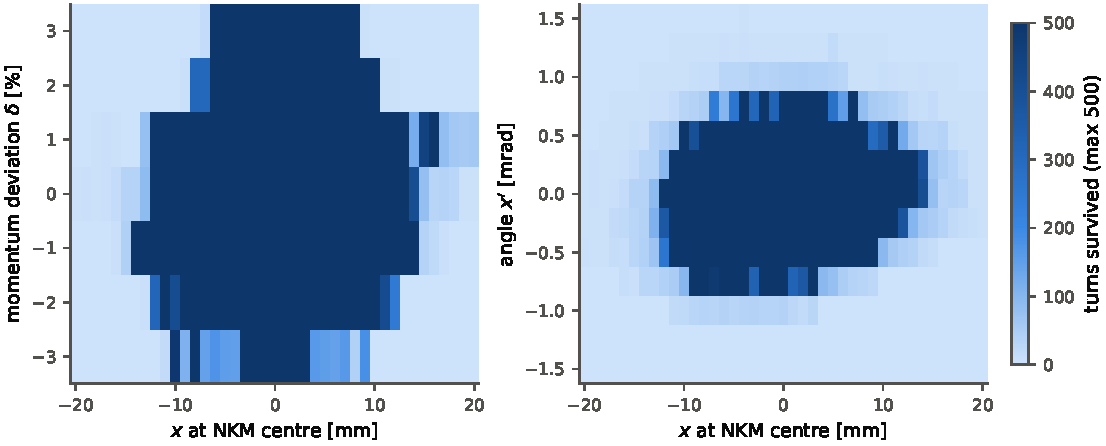
\includegraphics[width=0.95\textwidth]{generated/figures/fig2_dynamic_aperture.pdf}
\caption{Dynamic aperture at the NKM centre from native tracking of single particles for 500 turns (1\,mm grid in $x$): turns survived versus $x$ and momentum deviation at $x'=0$ (left) and versus $x$ and $x'$ at $\delta=0$ (right).}
\label{fig:da}
\end{figure}

\subsection{Kicker field and tracking}

The 0.525\,m four-loop magnet is a preliminary design for this study by Dong-Eon Kim (Pohang Accelerator Laboratory), as stated by the author; it is not the KLS baseline injection kicker. The baseline uses a four-kicker orbit bump and a 1\,mm thin septum~\cite{Hahn2024}. The alternative NKM scheme studied here retains an assumed 2\,mm blade and a stored-beam edge at $-16$\,mm; these are study geometry, not the published baseline septum. Loop powering has not been specified, so series and independent-loop cases are distinguished in the transparency tolerances.

The NKM consists of four closed rectangular filament loops, one per quadrant, each with an inner and an outer longitudinal wire joined by end connectors (figure~\ref{fig:geom}, left). The field of straight filaments in vacuum is evaluated in closed form (Biot--Savart), including the fringe and end-connector fields. Its straight-line integrals reproduce both components of the RADIA kick map to \MapAgreeRad\,rad (\MapAgreeRel\ relative) on \MapNodes\ nodes, so the RADIA calculation and the filament model describe the same field. The tabulated map stores $(\int B_y\,\mathrm{d}s, \int B_x\,\mathrm{d}s)/B\rho$; the curl-free kick pair, $\partial\Delta x'/\partial y=\partial\Delta y'/\partial x$, requires $-\int B_x\,\mathrm{d}s$ for the vertical kick. Using the map's vertical sign therefore turns vertical defocusing into focusing; all thin-kick results below use the corrected sign.

The magnet is tracked in 640 drift--kick--drift slices over $\pm0.45$\,m in canonical AT coordinates, $\mathrm{d}p_x/\mathrm{d}s = PS(B_y-y'B_s)/B\rho$ and $\mathrm{d}p_y/\mathrm{d}s=PS(-B_x+x'B_s)/B\rho$ with slopes $x'=p_x/(1+\delta)$, polarity $P$ and field scale $S$. The kick acts on canonical momentum and carries no $1/(1+\delta)$ factor; the exit angle changes by \DeltaSensUrad\,$\mu$rad per $10^{-3}$ in $\delta$. Slice and span refinement change the exit angle by less than \SliceConvRad\,rad. Particles within 1\,mm of a conductor are counted as lost; none was. The polarity is chosen so that the kick at $x<0$ cancels the angle of a beam travelling from the septum towards the axis (figure~\ref{fig:geom}, right).

\begin{figure}[htbp]
\centering
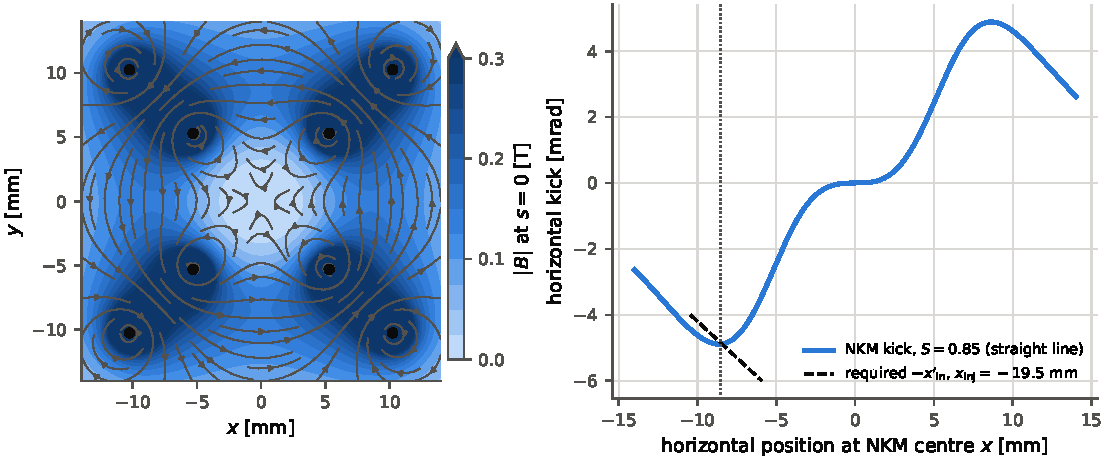
\includegraphics[width=0.95\textwidth]{generated/figures/fig1_nkm_geometry.pdf}
\caption{Left: NKM cross-section at $s=0$ with the wire positions, field lines and $|B|$ of the exact filament field. Right: straight-line horizontal kick at $y=0$ for $S=\OpScale$ and the kick required to cancel the incoming angle of a beam launched from the septum at $x_\mathrm{inj}=\OpXinjMm$\,mm; their intersection (dotted) is the thin-kick matched point.}
\label{fig:geom}
\end{figure}

An independent adaptive DOP853 integration checks the stated paraxial equations at the nominal point, the final interpolated angular edges (offsets \ODEEdgeLoMrad/\ODEEdgeHiMrad\,mrad), nonzero vertical position and angle, and $\delta=\pm0.002$. Relative/absolute tolerances are $2\times10^{-11}/2\times10^{-13}$. Maximum 640-slice discrepancies are $\ODEMaxX$\,m in $x$, $\ODEMaxPx$\,rad in $p_x$, $\ODEMaxY$\,m in $y$ and $\ODEMaxPy$\,rad in $p_y$. Refinement through 1280 slices and $\pm0.9$\,m spans is below one percent of a $0.1\sigma$ response in either plane. The field is exact for the filament geometry; tracking is a validated paraxial approximation.

\subsection{Injected beam, capture and controls}

The injected bunch is generated at booster extraction and tracked element by element through the matched BTS line to the septum exit, where it is placed at $(x_\mathrm{inj}, x'_\mathrm{inj})$. It drifts to the magnet, is tracked through the 3-D NKM once (single-turn pulse, section~\ref{sec:pulse}) and then for 500 turns. \emph{Capture} is the fraction of injected particles alive after the last turn; intervals are 95\,\% Wilson intervals~\cite{Wilson1927} for particles and cluster-bootstrap intervals for error realizations. Lost particles are classified as lost at septum creation, inside the magnet, at the septum on a later turn, or elsewhere in the ring; the categories reconcile with the particle count. The \emph{matched} angle is the inner root of zero centroid angle after the magnet. Two controls receive identical particles: a uniform \emph{dipole} kick and a \emph{linearised} kick (with its curl-free vertical partner), both calibrated to the 3-D response of the nominal centroid.

\section{Finite-length and vertical effects}
\label{sec:mechanism}

At the operating point of section~\ref{sec:window} the thin kick map gives a matched angle of \MatchThinMrad\,mrad, the 3-D magnet \MatchThreeDMrad\,mrad. To isolate the cause, the map's horizontal profile was distributed over the magnet length and sampled either along the undeflected straight line or along the self-consistent deflected path (figure~\ref{fig:mech}). Straight-path sampling gives \MatchStraightMrad\,mrad; the deflected path gives \MatchBentMrad\,mrad, equal to the 3-D result, and reproduces its response to angle errors to 0.01\,mm. The finite-length effect is therefore the beam's own deflection inside the magnet, with a sagitta $|K|L/8=\SagittaMm$\,mm, not path averaging or field details.

The effect is asymmetric. A positive septum angle error moves the trajectory inwards; on the straight line it would cross the kick extremum onto the weaker inner flank, leaving the extra angle under-compensated. The self-deflection instead holds the trajectory on the outer side of the extremum, where the kick is largest (figure~\ref{fig:mech}, centre). A $+0.3$\,mrad error changes the betatron amplitude of the kicked centroid by \AmpThinPlus\,mm with the thin kick but by \AmpThreeDPlus\,mm with the 3-D magnet, whereas $-0.3$\,mrad gives \AmpThinMinus\ and \AmpThreeDMinus\,mm; the nominal amplitude is larger (\AmpThreeDNom\ against \AmpThinNom\,mm). At fixed integrated kick, a longer magnet lowers the sensitivity to positive errors but raises the nominal amplitude, and for $L\geq\LengthNoMatchM$\,m no matched solution remains (figure~\ref{fig:mech}, right). A kick map is adequate only when the sagitta is small compared with the width of the kick extremum.

The vertical field matters as much. Near the kick extremum the 3-D magnet defocuses vertically: a centroid at $y=1$\,mm receives \VertKickThreeD\,mrad, against \VertKickThin\,mrad from the sign-corrected thin map, because the deflected path samples the field off the straight line. On identical bunches at the earlier operating point, capture is \CapThinLegacy\,\% with the map's original vertical sign, \CapThinPhys\,\% with the corrected sign and \CapThreeDRematch\,\% with the 3-D magnet. Suppressing only the 3-D vertical kick restores \CapThreeDNoVert\,\% (the horizontal-only finite-length model gives \CapThickOneD\,\%), so at that point the vertical defocusing costs about five percentage points. The linear vertical defocusing equals $-\partial\Delta x'/\partial x$ and vanishes at the kick extremum; at the operating point selected in section~\ref{sec:window}, where the centroid sits at the extremum, the cost is about two points (section~\ref{sec:survival}).

\begin{figure}[htbp]
\centering
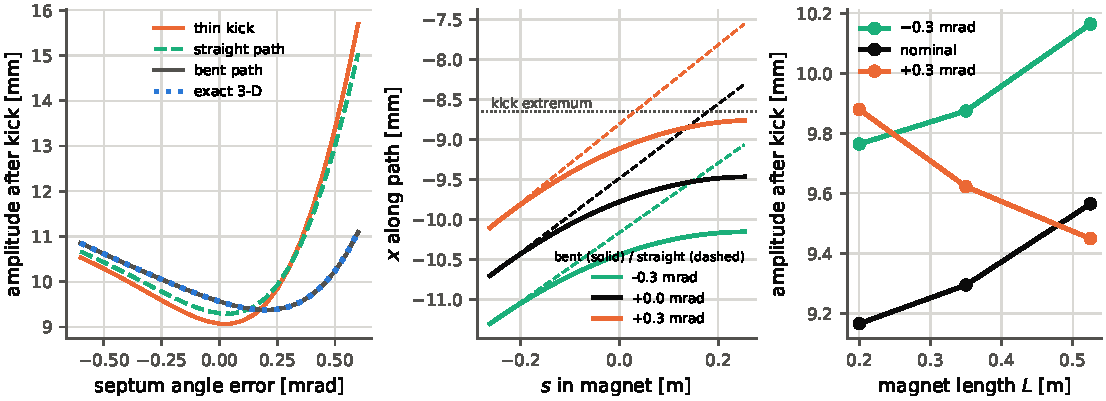
\includegraphics[width=\textwidth]{generated/figures/fig4_mechanism.pdf}
\caption{Finite-length mechanism. Left: betatron amplitude of the kicked centroid at the NKM centre versus septum angle error for the thin kick, the profile sampled on the straight and on the deflected path, and the exact 3-D field, each at its own matched angle. Centre: centroid path inside the magnet for angle errors of $-0.3$, 0 and $+0.3$\,mrad (solid: deflected; dashed: straight) relative to the kick extremum. Right: deflected-path model versus magnet length at fixed integrated kick.}
\label{fig:mech}
\end{figure}

\section{Operating window}
\label{sec:window}

At the final point and reference chamber, the native ring captures \FinalBackendNative\,\% at 500 turns, versus \FinalBackendLinear\,\% for an affine element-map reference on identical particles. The reference retains element lengths and explicit aperture checks at physical boundaries, and linearizes about the six-dimensional closed orbit with RF and radiation. A small-perturbation one-turn check agrees within $\FinalBackendTangentMax$ in the corresponding metre/radian/dimensionless coordinates. It deliberately omits nonlinear dynamics; all capture conclusions use native tracking.

Nominal native survival at 4000 turns is \FinalLong\,\% (95\,\% particle Wilson interval \FinalLongLo--\FinalLongHi\,\%), a loss of \FinalLateLoss\ percentage points after turn 500. The 500-turn prefix reproduces the paired chamber-study particle masks exactly. Fresh bunches at the interpolated lower and upper angular-edge candidates give \FinalLowerShort/\FinalUpperShort\,\% at 500 turns and \FinalLowerLong/\FinalUpperLong\,\% at 4000 turns (95\,\% intervals \FinalLowerLongLo--\FinalLowerLongHi\,\% and \FinalUpperLongLo--\FinalUpperLongHi\,\%). The degraded corrected ring 5501 gives \FinalDegradedShort\,\% at 500 turns and \FinalDegradedLong\,\% at 4000 turns (\FinalDegradedLongLo--\FinalDegradedLongHi\,\%). Thus the stated window remains a 500-turn conditional contour, not an infinite-time acceptance or a guaranteed 4000-turn 80\,\% contour.

\begin{figure}[htbp]
\centering
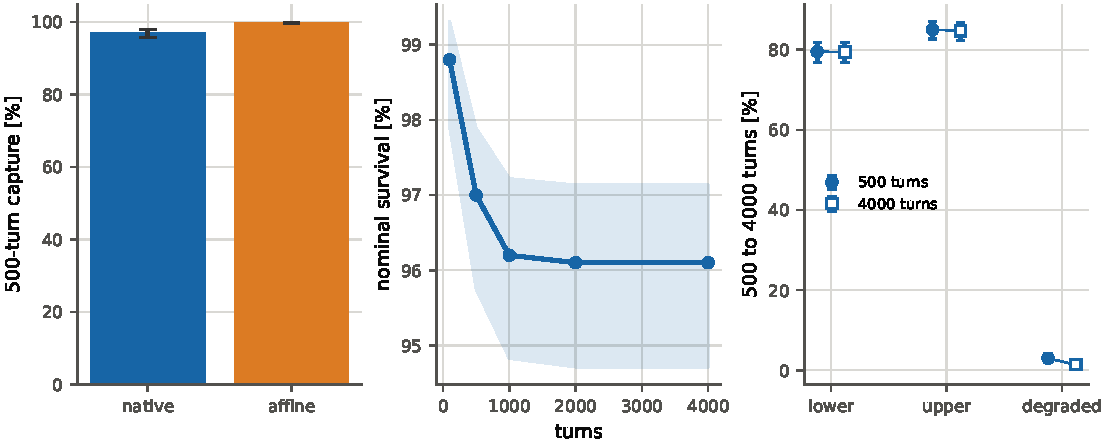
\includegraphics[width=\textwidth]{generated/figures/fig3_model_validation.pdf}
\caption{Final-point validation with the 3-D NKM, design beam and reference chamber. Left: native and affine-element backends at 500 turns on the same two 500-particle bunches (seeds 1001/1002; 95\,\% particle Wilson bars). Centre: native nominal survival with turn count (same particles; Wilson band). Right: 500-to-4000-turn survival for interpolated lower/upper angular-edge candidates and corrected ring 5501, each with two fresh 500-particle bunches (seeds 2001/2002); circles/squares denote 500/4000 turns, with 95\,\% Wilson bars. Intervals are conditional on the selected models and ring, not machine-population uncertainty.}
\label{fig:val}
\end{figure}

The point $x_\mathrm{inj}=\OpXinjMm$\,mm, $S=\OpScale$, $x'_\mathrm{inj}=\OpXpMrad$\,mrad was selected by the largest particle-Wilson lower bound in a fixed matched-point grid using a 100/10\,nm\,rad sensitivity beam. Four fresh bunches gave \ValThreeD\,\% (\ValThreeDLo--\ValThreeDHi\,\%) for that beam and septum-only aperture. This independent sample reduces reuse of selection noise; it does not remove dependence on the searched grid or model. The design-beam/chamber studies retain these knobs without reselection and therefore test a conditional operating point rather than a new global optimum.

We estimate the connected operating window above 80\,\% capture around that fixed point. Linear interpolation gives angle offsets from \FinalAngleLo\ to \FinalAngleHi\,mrad (width \FinalAngleWidth\,mrad), and position offsets span \FinalPositionLo\ to \FinalPositionHi\,mm (width \FinalPositionWidth\,mm). Each value uses seeds 1001/1002 and 500 particles per seed. A fixed 0.2\,mm/mrad grid is extended if a boundary remains above threshold, with a maximum offset of 3; crossing cells are refined once to 0.1 spacing and linearly interpolated. Grid resolution is not a confidence interval for a crossing. The long-turn edge checks use fresh particles and do not redefine the selected 500-turn window.

\begin{figure}[htbp]
\centering
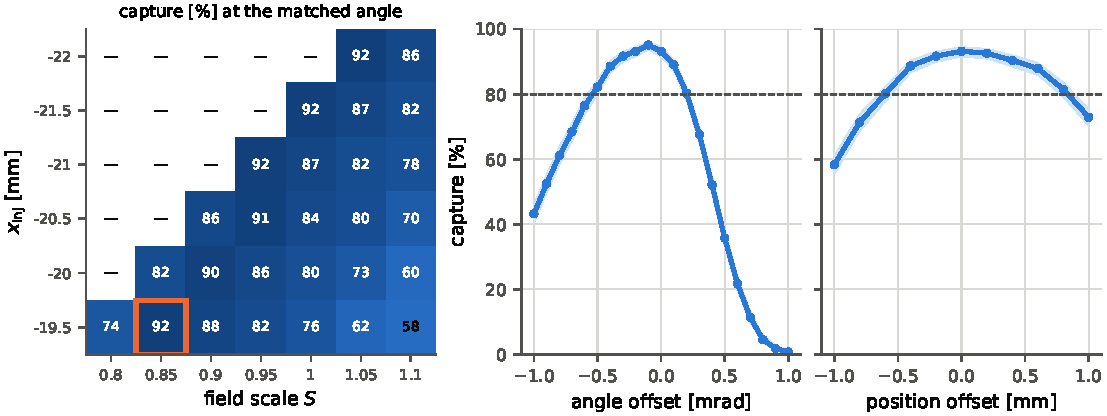
\includegraphics[width=\textwidth]{generated/figures/fig5_operating_window.pdf}
\caption{Design-beam operating window with the reference chamber and fixed NKM settings. Left/right: capture versus septum-exit angle/position offset, 500 native turns, two 500-particle bunches (seeds 1001/1002) per point. Bands are conditional 95\,\% particle Wilson intervals; the dashed line marks 80\,\%. Crossing cells have 0.1\,mrad/mm spacing after refinement.}
\label{fig:window}
\end{figure}

\section{Survival, acceptance and sensitivity}
\label{sec:survival}

Tracking \SurvN\ particles for \SurvTurns\ turns (seeds \SurvSeeds), about one damping time, \SurvShort\,\% survive 500 turns, \SurvMid\,\% survive 2000 turns and \SurvLong\,\% the full run (95\,\% particle Wilson interval \SurvLongLo--\SurvLongHi\,\%, conditional on these two bunches); \SurvLateLossPct\,\% of the particles are lost after turn 500 (figure~\ref{fig:accept}, right). A single \BigN-particle bunch gives \BigCap\,\% (\BigLo--\BigHi\,\%): \BigLossSeptumReturn\ particles are lost at the septum on later turns, \BigLossElsewhere\ elsewhere in the ring, \BigLossCreation\ at creation and \BigLossMagnet\ inside the magnet. With a uniform rectangular chamber of half-height 5\,mm and half-width 15, 12, 11 or 10\,mm at every element, capture is \AperFifteenCap, \AperTwelveCap, \AperElevenCap\ and \AperTenCap\,\%, respectively. The loss at 15\,mm is vertical: a 10\,mm half-height restores \AperDiagYten\,\%, and an open horizontal aperture with a 5\,mm half-height gives \AperDiagXopen\,\%. On the same particles the 5\,mm half-height costs the same with and without the NKM vertical kick (\AperDiagRef\ to \AperDiagXopen\,\% and \AperDiagOpenNoVert\ to \AperDiagNoVert\,\%), which is consistent with horizontal-to-vertical transfer in the ring; no unique coupling resonance is diagnosed here. At the selected point the NKM vertical kick itself costs only the difference between \AperDiagOpenNoVert\ and \AperDiagRef\,\%, less than at the earlier point of section~\ref{sec:mechanism}, because the centroid now sits near the kick extremum, where the linear vertical focusing term $-\partial\Delta x'/\partial x$ vanishes. The vertical stay-clear at large horizontal amplitude is therefore a design constraint of the injection straight. Random relative gradient errors of \RingErrLowRel\,\% and \RingErrHighRel\,\% on all quadrupoles and \RingErrSextRel\,\% on all sextupoles (\RingErrLowSeeds\ seeds each, no misalignments, no correction) reduce the negative DA edge to between \RingErrLowDAmin\ and \RingErrLowDAmax\,mm and between \RingErrHighDAmin\ and \RingErrHighDAmax\,mm, and give mean capture \RingErrLowMean\,\% (range \RingErrLowMin--\RingErrLowMax\,\%) and \RingErrHighMean\,\% (\RingErrHighMin--\RingErrHighMax\,\%). Because these errors are uncorrected, they define selected sensitivity scenarios rather than predict a corrected machine; the injection DA of the corrected KLS lattice is the decisive input for an operational estimate.

\begin{figure}[htbp]
\centering
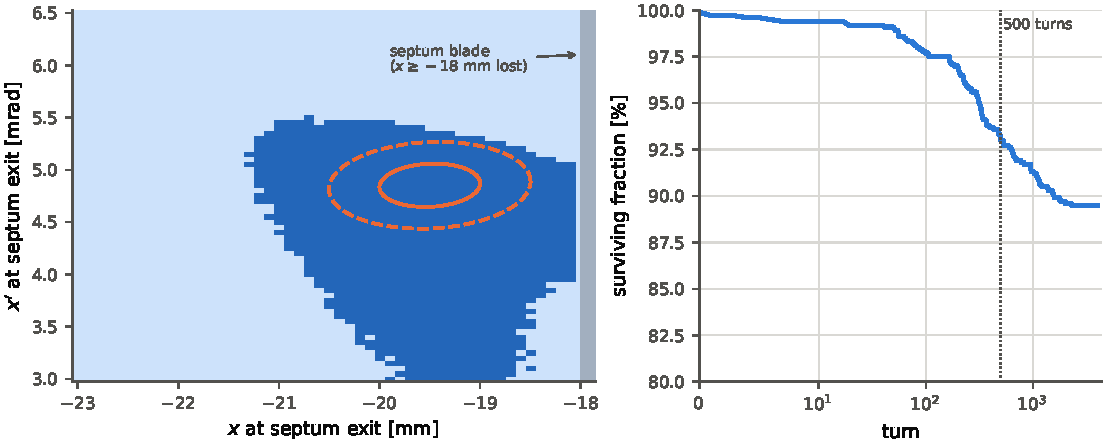
\includegraphics[width=\textwidth]{generated/figures/fig6_acceptance_survival.pdf}
\caption{Left: single-particle survival for 500 turns in septum phase space ($\delta=0$, \AccPoints\ particles) with the injected-beam 1$\sigma$ (solid) and 2$\sigma$ (dashed) ellipses and the septum blade (grey). Right: surviving fraction of the injected bunch versus turn at the selected point.}
\label{fig:accept}
\end{figure}

A separate selected corrected-ring scenario applies correlated 30\,$\mu$m girder offsets, 30\,$\mu$m independent magnet offsets, 100\,$\mu$rad rolls, gradient/sextupole errors and skew-quadrupole components, all explicit sensitivity assumptions. Ten seeds (5501--5510) use the 120 HVC correctors and BPM markers with a truncated-SVD response, followed by bounded Q11/Q12 tune correction. The selected rms criterion is 100\,$\mu$m; an earlier 20\,$\mu$m target was not attained. Maximum achieved BPM rms residuals are \ScenOrbitXmax/\ScenOrbitYmax\,$\mu$m, and the largest fractional-tune residual is \ScenTuneMax. The full DA grids (figure~\ref{fig:correctedring}) define the subsequent chamber/error scenario; they are not a commissioned-machine prediction.

\begin{figure}[htbp]
\centering
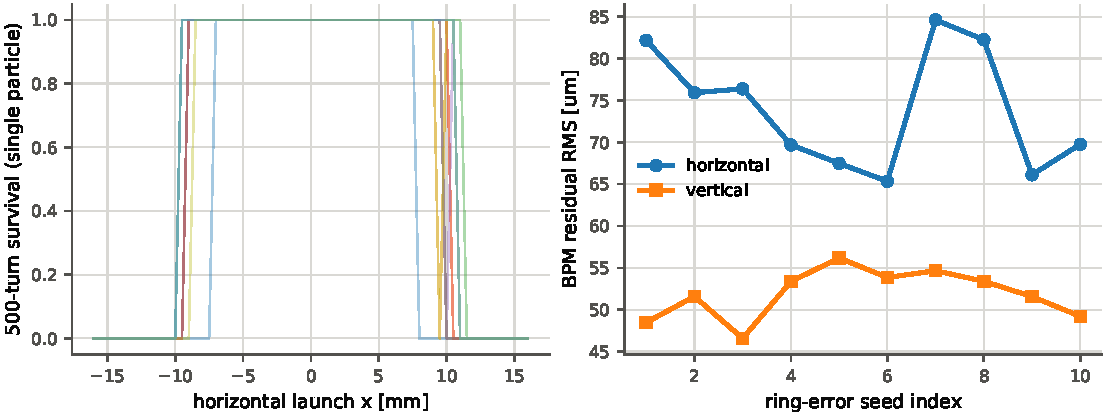
\includegraphics[width=\textwidth]{generated/figures/fig10_corrected_ring.pdf}
\caption{Selected corrected-ring scenario, ten fixed seeds. Left: deterministic 500-turn native survival on a 0.5\,mm horizontal launch grid, with RF/radiation and the reference chamber. Blue/white cells denote surviving/lost launches. First failed grid points are not exact stable edges. Right: horizontal and vertical BPM rms residuals after SVD orbit and bounded tune correction. Curves show seed variation, without a particle-sampling interval.}
\label{fig:correctedring}
\end{figure}

The chamber reference uses arc half-width/height 12/9\,mm, centre-bend half-height 4.87\,mm, and an inscribed ellipse where the octagonal corners are unspecified. An assumed rectangular NKM straight has half-width/height 30/15\,mm. Nineteen identified ordinary straights receive 3\,m IVU segments; their assignment is a scenario, not a surveyed map. The reference open half-gap is 9\,mm; a 2.5\,mm closed magnetic half-gap is a stress case and does not account for a liner. The separate incoming transport retains its source lattice and septum creation cut; its chamber has not been surveyed for this alternative injection scheme.

For the 7.67\,nm\,rad design booster beam, the reference chamber gives \ChamberNom\,\% capture at 500 turns (95\,\% particle Wilson interval \ChamberNomLo--\ChamberNomHi\,\%; two 500-particle bunches, seeds 1001/1002). The paired dipole gives \ChamberDipole\,\%; the NKM-minus-dipole difference is \ChamberDiff\ percentage points (95\,\% paired-particle bootstrap interval \ChamberDiffLo\ to \ChamberDiffHi; 10\,000 draws, seed 1729). Arc half-widths 10, 12 and 15\,mm give 81.7, 97.0 and 99.7\,\% at each tested half-height (4.87, 7.5, 9\,mm). Thus 10\,mm is the smallest tested width exceeding 80\,\% in this ideal-ring sample, while 12\,mm retains the reference result; neither is a continuous minimum or a machine tolerance. Across the ten corrected rings, mean capture is \ChamberRingMean\,\%, median \ChamberRingMedian\,\%, tenth percentile \ChamberRingPten\,\%, and range \ChamberRingMin--\ChamberRingMax\,\%. These are different descriptors of a finite scenario population.

\begin{figure}[htbp]
\centering
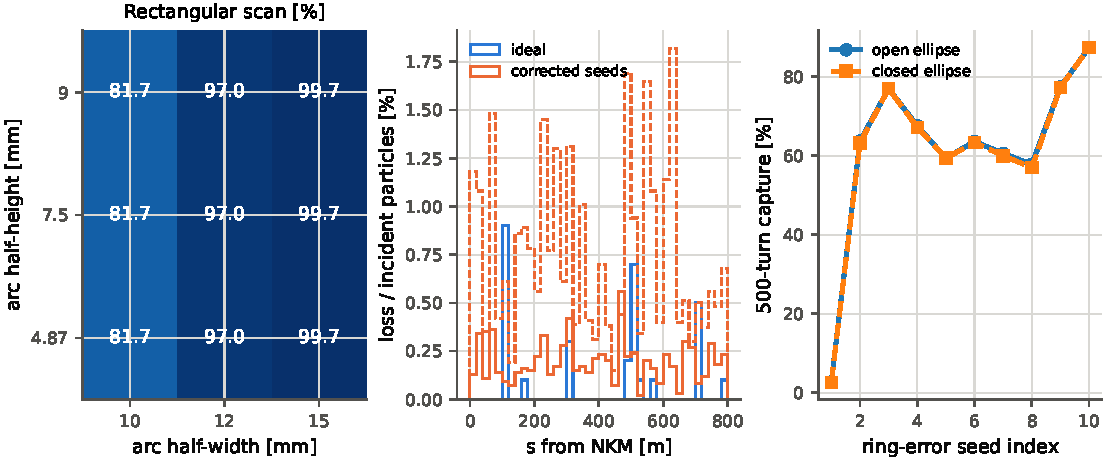
\includegraphics[width=\textwidth]{generated/figures/fig11_chamber.pdf}
\caption{Declared chamber with the design booster beam, 500 native turns and two seeds of 500 particles per ring/profile/model. Left: ideal-ring capture versus arc half-apertures, with other region limits retained. Centre: ring losses per incident particle in 20\,m bins from the NKM centre; solid/dashed/dotted denote horizontal/vertical/dynamical losses. For elliptic apertures the larger normalized coordinate defines the plane. Right: capture for each corrected ring with open and closed IVUs. Points are conditional sample fractions; the loss histograms and finite ring-seed variation have no assigned confidence band.}
\label{fig:chamber}
\end{figure}

\section{Stored-beam transparency}
\label{sec:transparency}

The kick of the four-loop magnet is odd in $x$ on the midplane and its near-axis expansion has a leading cubic term, $\Delta x'\simeq c_3x^3$ with $c_3={}$\CubicCoeff\,rad\,m$^{-3}$ at $S=\OpScale$. For an aligned kicker and a centred, symmetric Gaussian beam the ideal centroid kick therefore vanishes exactly. This does not imply unchanged finite-beam moments: deterministic quadrature gives single-pass projected emittance changes of \AlignedMomentX\ horizontally and \AlignedMomentY\ vertically. Orders 20, 40 and \MomentGHOrder\ per axis agree at the reported precision. The meaningful quantities are the response to an offset between kicker and stored orbit and the emittance change, evaluated deterministically from the exact field by Gauss--Hermite quadrature (figure~\ref{fig:transp}, right). Offsets of 0.1, 0.2 and 0.5\,mm give centroid amplitudes $A_x$ of \TranspOneAmp, \TranspTwoAmp\ and \TranspFiveAmp\ of the rms size, and the spread of the kick across the beam increases the emittance about the displaced centroid by \TranspOneEmit, \TranspTwoEmit\ and \TranspFiveEmit; a 0.2\,mm vertical offset gives \TranspVertTwoAmp\ of the vertical rms size. Once the centroid oscillation has also filamented, the rms emittance grows by the factor $1+A_x^2/2+\Delta\varepsilon_x/\varepsilon_x$, i.e.\ \TranspTwoTotal\ at 0.2\,mm and \TranspFiveTotal\ at 0.5\,mm. Native tracking uses two seeds (11 and 12), each with 300 paired particles, with radiation on. The maximum centroid difference is measured at the ends of turns 1--50, and projected emittance at the end of turn \TrackedTurns: $A_x/\sigma_x=\TrackedTwoAmp$ and \TrackedFiveAmp, and mean paired emittance ratios \TrackedTwoEmitRatio\ and \TrackedFiveEmitRatio. These tracked observables need not equal a fully filamented analytic estimate. An offset of 0.2\,mm thus keeps the stored-beam disturbance at about a tenth of its size, whereas 0.5\,mm is not transparent. The bicubic interpolation of the map agrees with the exact field to \BicubicErr\,rad near the axis, whereas bilinear interpolation errs by \BilinearErr\,rad and overstates the 0.1\,mm response nineteen-fold (\TranspBilinOne). The calibrated dipole control would displace the stored beam by about \CtrlDipoleAmp\ rms sizes in a linear estimate; this hypothetical figure only illustrates why a uniform kicker cannot be used for top-up.

The assumed vertical-to-horizontal emittance ratio is 0.10, as supplied by the author; for a fixed vertical dipole kick, $A_y/\sigma_y\propto\varepsilon_y^{-1/2}$. Individual wire displacements and independent loop-current errors break the cancellation (tables~\ref{tab:wiretol} and \ref{tab:looptol}). The one-error-at-a-time wire limits range from \WireTolMin\ to \WireTolMax\,$\mu$m for both centroid amplitudes to remain below 0.1\,$\sigma$. Independent loop currents require relative balance of about \LoopTolerance. In series powering, a common current error preserves dipole cancellation provided the geometry remains symmetric; geometry errors still matter. These are local linear tolerances, not an allocation for simultaneous errors or a manufacturing specification.

\begin{table}[htbp]
\centering\footnotesize
\caption{On-axis wire sensitivity. Wire numbers follow the four quadrant loops, inner then outer wire. $u$ is the displaced coordinate. Dipole derivatives $D_{x,y}=\partial K_{x,y}/\partial u$ are in rad/m; $Q_n=\partial J_{xx}/\partial u$ and $Q_s=\partial J_{xy}/\partial u$ are in rad/m$^2$, with $J=\partial(K_x,K_y)/\partial(x,y)$, $J_{yy}=-J_{xx}$ and $J_{yx}=J_{xy}$ to numerical precision. $t_x,t_y$ are single-error 0.1-sigma limits in $\mu$m. A dash indicates no resolved first-order dipole sensitivity; higher orders remain. Deterministic central differences, step 0.1\,$\mu$m; no statistical interval.}
\label{tab:wiretol}
\begin{tabular}{rrrrrrrr}\toprule
Wire & $u$ & $D_x$ & $D_y$ & $Q_n$ & $Q_s$ & $t_x$ & $t_y$\\\midrule
\WireSensitivityRows
\bottomrule\end{tabular}
\end{table}

\begin{table}[htbp]
\centering\small
\caption{Independent-loop relative-current sensitivity. Dipole derivatives are in rad per relative current; normal and skew quadrupole derivatives are in rad/m per relative current. The final column is the joint two-plane 0.1-sigma single-loop limit in units of $10^{-4}$. Deterministic derivatives with relative-current step $10^{-5}$; no statistical interval.}
\label{tab:looptol}
\begin{tabular}{rrrrrr}\toprule
Loop & $D_x$ & $D_y$ & $Q_n$ & $Q_s$ & Limit\\\midrule
\LoopSensitivityRows
\bottomrule\end{tabular}
\end{table}

\begin{figure}[htbp]
\centering
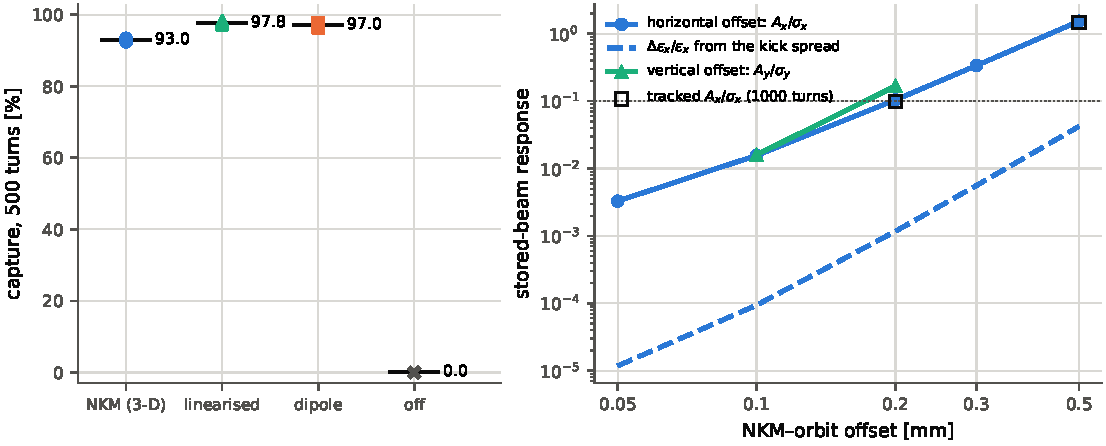
\includegraphics[width=\textwidth]{generated/figures/fig7_controls_transparency.pdf}
\caption{Left: 100/10\,nm\,rad sensitivity case with the septum aperture and no additional chamber; four fresh 500-particle bunches at the selected point for the 3-D NKM, the calibrated linearised and dipole controls and the kicker off (markers: bunches; bars: mean). The inset shows per-bunch NKM-minus-dipole differences (dots), their mean (square) and a paired-bunch bootstrap 95\,\% interval (10\,000 resamples, seed 1729; only four bunches). Right: deterministic centroid amplitude and filamented emittance growth versus NKM-to-orbit offset. Open squares are the mean of two 300-particle tracked seeds, using maximum centroid differences over ends of turns 1--50; they are not 1000-turn amplitudes. Emittance ratios in the text use the end of turn 1000. No sampling interval is assigned to deterministic quadrature.}
\label{fig:transp}
\end{figure}

The controls (figure~\ref{fig:transp}, left) separate the cost of nonlinearity: the linearised and dipole kicks capture \ValLinear\ and \ValDipole\,\%, the paired NKM-minus-dipole difference is \ValDiffDipole\ points (95\,\% paired-bunch bootstrap interval \ValDiffDipoleLo\ to \ValDiffDipoleHi), conditional on this larger-emittance sample; with the kicker off no particle survives.

\section{Robustness and tolerances}
\label{sec:robust}

\subsection{Error budget}

Table~\ref{tab:errors} lists the assumed errors. They are design hypotheses, not component specifications; static errors are drawn once per realization, the booster centroid, energy and NKM amplitude and timing errors represent shot-to-shot jitter. Timing jitter is represented as a field-scale change that gives the same kick change for the injected centroid; unlike an additive dipole kick it leaves the field zero on axis. With the matched BTS optics fixed, \TolN\ realizations give a median horizontal exit mismatch $M_x=\tfrac12\mathrm{Tr}(\Sigma_0^{-1}\Sigma)-1$ (zero for matched Twiss parameters; $\Sigma$, $\Sigma_0$ the normalised beam matrices at the BTS exit and its target) of $\TolMedianMx\times10^{-3}$ (95\,\% interval \TolMedianMxLo--\TolMedianMxHi$\times10^{-3}$), and \TolFailures\ exceed the 60\,m $\beta$ limit; this optics metric alone does not quantify capture loss.

\begin{table}[htbp]
\centering
\caption{Historical rms errors (Gaussian, untruncated) of the campaign-02 ensembles. Values are assumptions, not measured specifications; the finalized campaign-03 budget is described below.}
\label{tab:errors}
\small
\begin{tabular}{@{}lll@{}}
\toprule
Booster centroid jitter (shot-to-shot) & \BudJitX\,mm, \BudJitXp\,mrad & sensitivity assumption \\
Booster $\beta$ mismatch, emittance, energy & \BudBetaMis\,\%, \BudEmit\,\%, \BudEnergy\,\% & sensitivity assumption \\
Energy-spread variation & $\BudEspread\times10^{-4}$ & sensitivity assumption \\
BTS quadrupole gradient, offset, roll & \BudQuadK\,\%, \BudQuadDx\,$\mu$m, \BudQuadRoll\,mrad & sensitivity assumption \\
BTS dipole field & \BudDipB\,\% & sensitivity assumption \\
Septum position & \BudSeptum\,mm & sensitivity assumption \\
NKM amplitude, timing (as field scale), offset & \BudNkmScale\,\%, \BudNkmTiming\,$\mu$rad equiv., \BudNkmDx\,mm & sensitivity assumption \\
Ring closed orbit at NKM & \BudRingCo\,mm & sensitivity assumption \\
\bottomrule
\end{tabular}
\end{table}

For the final campaign the booster design values are $\varepsilon_x=7.67$\,nm\,rad and $\sigma_\delta=0.00106$~\cite{Lee2024}, with an assumed vertical ratio of 0.10. Extraction orbit jitter and septum current stability are not public. The final budget therefore parametrizes them and adds separate thin-septum strength jitter (0.1\,\% relative about the published 10\,mrad bend~\cite{Hahn2024}), RF phase (0.001\,rad) and arrival relative to NKM firing (2\,ns rms). These three rms values are explicit sensitivity assumptions. At the lattice RF frequency of 499.593\,MHz, phase shifts the injected longitudinal coordinate by $c\Delta\phi/(2\pi f_\mathrm{RF})$; the independent pulse-relative timing samples a 5.3\,$\mu$s half-sine at peak phase without another longitudinal-coordinate shift. The legacy equivalent transverse timing kick is disabled in the final budget. Alignment and strength values in table~\ref{tab:errors} test sensitivity rather than represent construction specifications; their roles and the retained unmodelled terms are recorded in the budget supplement.

\subsection{Combined errors and tolerance curves}

Two ensembles bound the treatment of static transfer-line errors. Without orbit correction, the static trajectory errors of the transfer line reach the septum; with ideal steering at the septum exit, the static trajectory of each perturbed line is removed and shot-dependent errors and uncorrected static optics, vertical orbit and kicker/septum offsets remain. Over \RobN\ realizations from three seeds (200 particles, 500 turns), the 3-D NKM captures \RobMean\,\% on average without correction (\RobMeanLo--\RobMeanHi\,\%, median \RobMedian\,\%) and \RobCMean\,\% with correction (\RobCMeanLo--\RobCMeanHi\,\%, median \RobCMedian\,\%), against \RobDipMean\ and \RobCDipMean\,\% for the dipole control on the same realizations (paired differences \RobNkmMinusDip\ and \RobCNkmMinusDip\,points, 95\,\% intervals \RobNkmMinusDipLo\ to \RobNkmMinusDipHi\ and \RobCNkmMinusDipLo\ to \RobCNkmMinusDipHi); the realization without errors captures \RobZeroErr\,\% (dipole \RobZeroErrDip\,\%) (figure~\ref{fig:robust}, left). The deficit with respect to the dipole thus grows from about two points without errors to about twenty with them: the NKM kick falls off on both sides of its extremum, so its angular window (section~\ref{sec:window}) is narrower than that of the uniform kick, and realizations whose transfer-line exit angle deviates by more than 0.2\,mrad lose most. Controlling for all other sampled errors (partial rank correlation), the booster angle jitter is the dominant driver for both kickers ($\rho=-0.45$ for the NKM and $-0.68$ for the dipole without correction, $-0.52$ and $-0.75$ with it); once the static offset is corrected, the booster position jitter also becomes significant ($\rho=-0.24$ for both).

Scaling only the booster centroid jitter on paired realizations (figure~\ref{fig:robust}, centre) separates jitter from static errors. With correction, the mean capture is \JitCFullMean\,\% at the assumed jitter, \JitCHalfMean\,\% at half, \JitCQuarterMean\,\% at a quarter and \JitCZeroMean\,\% without jitter; below a quarter of the assumed amplitude (0.125\,mm, 0.05\,mrad) the jitter has a difference unresolved at the available precision. Position jitter alone gives \JitCXOnlyMean\,\% and angle jitter alone \JitCXpOnlyMean\,\%. Without correction, removing the jitter raises the mean only to \JitZeroMean\,\%, because the static transfer-line errors displace the exit centroid by 0.7\,mm rms, more than the position window. Even with correction and without jitter the mean stays below 80\,\% (median \JitCZeroMedian\,\%, \JitCZeroFracEighty\,\% of realizations above 80\,\%): the remaining loss comes from the combined static errors of table~\ref{tab:errors} (kicker, orbit and septum offsets, energy and dipole-field errors), none of which dominates. A mean capture of 80\,\% under this budget therefore needs, besides orbit correction and booster jitter of at most a quarter of the assumed value, either tighter static tolerances or a wider window, for example from sextupole optimisation for the injection DA. Without other errors, capture varies between \OffCapMin\ and \OffCapMax\,\% for NKM-to-orbit offsets within $\pm\OffRangeMm$\,mm, and from \EmitTwentyFiveCap\,\% at an injected emittance of 25\,nm\,rad to \EmitTwoHundredCap\,\% at 200\,nm\,rad.

\begin{figure}[htbp]
\centering
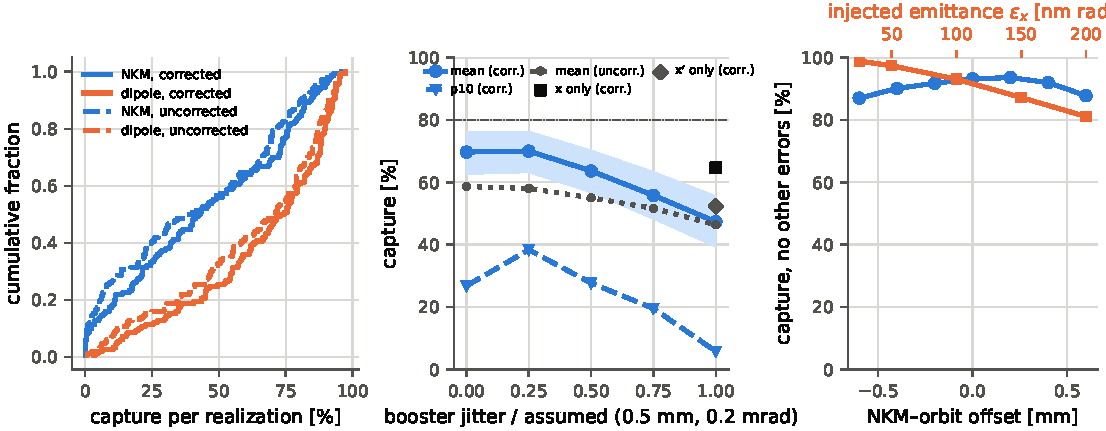
\includegraphics[width=\textwidth]{generated/figures/fig8_robustness.pdf}
\caption{Left: capture per error realization for the 3-D NKM and the calibrated dipole (three seeds). Solid: ideal static orbit correction of the transfer line; dashed: no correction. Centre: mean and 10th-percentile capture with correction versus the booster-jitter scale on paired realizations (seed 42, 50 per level; band: bootstrap 95\,\% of the mean), the mean without correction (dotted) and position-only and angle-only jitter with correction. Right: capture without other errors versus the NKM-to-orbit offset (blue, lower axis) and the injected emittance (orange, upper axis).}
\label{fig:robust}
\end{figure}

Ideal static steering transports the zero-input reference through each perturbed BTS, giving $(r_x,r_{p_x})$, then translates every bunch particle by $(x,p_x)\mapsto(x-r_x,p_x-r_{p_x})$ at the septum exit. The other four coordinates are unchanged. Booster shot jitter, vertical offsets, optics distortion, and kicker, ring-orbit and septum errors remain. This ideal translation does not represent a fitted orbit-correction system. Each realization draws static and shot-dependent variables once, so the reported bootstrap describes their joint distribution, not repeated shots on fixed machines.

\section{Pulsed-magnet considerations}
\label{sec:pulse}

The results above apply to an ideal single-pass spatial field. Native tracking of the nominal centroid observes positions \TurnOneXmm, \TurnTwoXmm\ and \TurnThreeXmm\,mm after turns 1--3 at the NKM centre. The corresponding straight-line full-field kicks are \TurnOneKickMrad, \TurnTwoKickMrad\ and \TurnThreeKickMrad\,mrad. Assigning one tenth of the conditional angular-window width (\ResidualAllowMrad\,mrad) as a residual allowance is a design assumption; it gives first/second-return fractional limits \ResidualTurnOne/\ResidualTurnTwo.

For a half-sine of total duration $\tau$, injection at its peak ($t=\tau/2$) gives subsequent field fraction $\max[0,\cos(\pi T_0/\tau)]$, with finite support. The native-centroid allowance gives $\tau\leq\PeakPhaseMaxPulseUs\,\mu$s; zero field on every return requires $\tau\leq\NoReturnMaxPulseUs\,\mu$s. A 5.3\,$\mu$s peak-phase example meets the latter condition, whereas 8\,$\mu$s retains \EightUsResidual\ of the peak on the first return. Deterministic timing offsets obey $1-\cos(\pi\Delta t/\tau)$, giving \TimingLossMin--\TimingLossMax\ for 1--5\,ns and 5--8\,$\mu$s. The 2\,ns Gaussian rms in the error model is a distribution, not a hard timing bound.

A train with its first bunch at the peak samples less field on later bunches: for the 5.3\,$\mu$s example, 100, 200 and 500\,ns train durations give approximately 0.18, 0.70 and 4.4\,\% variation. At an offset kicker the stored-beam centroid response scales with that field; aligned centroid cancellation does not imply zero finite-beam moment change. On-axis residual dipole and gradient allowances are \DipoleResidualRel\ and \GradResidualRel\ of the corresponding peak quantities. A hypothetical thin cylindrical conducting shell has diffusion time $\tau_\mathrm{eddy}\simeq\mu_0\sigma a t/2$: at $a=15$\,mm, a 1\,$\mu$m coating with $\sigma=10^6$\,S/m gives 9.4\,ns, whereas a 1\,mm wall with $\sigma=5\times10^7$\,S/m gives 0.47\,ms. These are order-of-magnitude scenarios, not predictions for the unspecified NKM chamber. Coating-induced multipoles require chamber-specific analysis~\cite{Kallestrup2019}; no time-dependent capture or operational pulse feasibility is claimed.

The sagitta ratio $\eta=|K|L/(8w)$ compares trajectory displacement with the horizontal kick-lobe full width at half maximum $w$. Figure~\ref{fig:generality} varies length, integrated strength and a second wire family scaled transversely by 1.25. It is a deterministic model comparison, not a universal capture criterion. A sliced vector map retains self-deflection and the physical vertical kick; the local focusing sign changes between flanks of the kick extremum. The original vertical-sign error was an input error, not a failure inherent to kick maps. Capture controls throughout are paired model comparisons on identical particles, not independently optimized injection systems.

\begin{figure}[htbp]
\centering
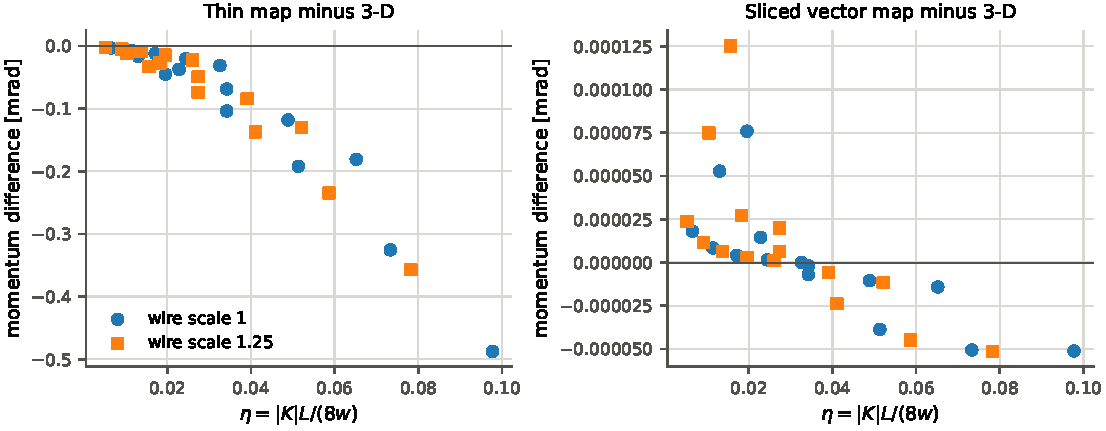
\includegraphics[width=\textwidth]{generated/figures/fig9_generality.pdf}
\caption{Single-centroid momentum differences versus $\eta$ for five lengths (0.2--1.0\,m), three integrated strengths and two transverse wire families. Left: thin vector map minus 3-D field. Right: vector map distributed over 1280 slices minus the 3-D field. Width $w$ is the negative kick lobe's full width at half maximum. The centroids have nonzero vertical position and angle; these deterministic comparisons have no sampling interval.}
\label{fig:generality}
\end{figure}

\section{Discussion and limitations}
\label{sec:discussion}

Four results generalise beyond this design. First, the kick map is not a controlled description of a strongly nonlinear injection kicker: the self-deflection inside the magnet, with sagitta $|K|L/8$, shifts the matched angle and changes the error sensitivity in a sign-dependent way, and the magnet length is a design variable that trades nominal amplitude against tolerance. Second, the curl-free vertical kick defocuses the injected bunch wherever the horizontal kick gradient is non-zero and costs up to several points of capture, which favours placing the centroid at the extremum; tabulated maps should be checked for $\partial\Delta x'/\partial y=\partial\Delta y'/\partial x$. Third, the transparency of an aligned NKM is a symmetry property; the engineering quantities are the kicker-to-orbit alignment, the on-axis residual field and the pulse length. Fourth, with an angular window of order \WinAngleWidth\,mrad and a position window of about \WinPosWidth\,mm, the injected orbit at the septum, not the kick strength or the transfer-line optics, decides whether the window can be used: static transfer-line errors must be corrected, the booster jitter kept to a quarter of the assumed amplitude, and the remaining static offsets of kicker, orbit and septum budgeted together.

The limitations are explicit. The ring is an ideal lattice; ring errors and apertures enter only as selected sensitivity scenarios. The filament model contains no iron, chamber or eddy-current fields and no pulse time dependence. The error budget is assumed. Capture is survival over 500 turns, checked to one damping time at the selected point. As at BESSY~II and SIRIUS~\cite{Gora2023,Velloso2023}, sextupole optimisation for the injection DA is expected to enlarge the window and was not attempted.

The corrected quarter-minus-zero jitter difference is $\QuarterPairedDiff$ percentage points (95\,\% paired percentile-bootstrap interval $\QuarterPairedLo$ to $\QuarterPairedHi$; \QuarterPairs\ realizations, 10\,000 resamples, seed 1729). A declared one-percentage-point loss margin is not supported by this interval. Thus 0.125\,mm and 0.05\,mrad are conditional candidate targets, not a demonstrated joint error allocation. At quarter jitter, mean \QuarterMean\,\%, median \QuarterMedian\,\%, tenth percentile \QuarterPten\,\% and fraction above 80\,\% of \QuarterAboveEighty\,\% describe distinct observables. Partial-rank associations are tested with Holm correction over all sampled-error variables; these are model-conditioned associations, not causal rankings.

\section{Conclusions}
\label{sec:conclusions}

For a 0.525\,m wire NKM in the 4\,GeV KLS design lattice, exact 3-D field tracking with a coupled transfer line gives \ValThreeD\,\% capture at the selected point (\ValDipole\,\% for an equally strong uniform kick), an angular window of \WinAngleWidth\,mrad at \WinThreshold\,\% capture, and an ideal centroid kick that vanishes for the aligned kicker and is \TranspTwoAmp\ of the rms size at a 0.2\,mm offset. A single thin map neglects self-deflection; vector maps can retain the vertical kick, whose original sign error is an input-convention error. Both corrections change capture by several points. Under the assumed errors the mean capture is \RobCMean\,\% with ideal static orbit correction and \RobMean\,\% without; the quarter-jitter result is precision-limited relative to zero jitter, and a mean capture of 80\,\% additionally requires tighter static tolerances or a wider window.

\section*{Data, software and code availability}

{\sloppy The simulation code, configurations and analysis scripts are available in the nkm-injection repository (\url{https://github.com/cspark7701/nkm-injection}). The figures and numbers are generated from the campaign artifacts listed, with SHA-256 digests, in \texttt{figure\_provenance.csv} of the manuscript directory \texttt{docs/\allowbreak paper/\allowbreak generated}. A frozen evidence bundle with the selected simulation outputs, input files, code snapshot and rebuild instructions is provided to referees; an archived release with a persistent identifier will be created on acceptance.\par}

\section*{Acknowledgments}

The author thanks the accelerator physics group at Korea University. Generative AI assistance (Anthropic Claude, used through Claude Code) was used to implement simulation drivers and the field model, run the campaigns, audit references and draft parts of the manuscript; all results were checked and the author takes full responsibility for the content.

\bibliographystyle{unsrt}
\bibliography{paper}

\end{document}
